\section{Calorimetry Jets}
\label{calo_jets}

In addition to finding jets in the tracking system, ECCE's full hermetic coverage can be used to measure the energy of the charged and neutral fraction of jets.  Like in the tracking analysis, this was done with 18x275 GeV Pythia 8 electron proton collisions with a $Q^2>100\hbox{ GeV}^2$ in the prop.4 configuration.  Once again, the anti-$k_T$ jet finding algorithm was used with a jet radius $R=0.5$ with the constraint $z<0.95$.  The electromagnetic and hadronic calorimeters are used together to identify jets.

To improve the collection of energy in the calorimeters, the towers are group together with clustering algorithms to try to make each cluster contain all the energy of a single particle.  Two algorithms in particular have been utilized in this analysis, V3 and MA clustering.

V3 clustering works by starting a cluster at the most energetic tower, and adding its cardinal neighbors to it if they have less energy, but still greater than a aggregation energy parameter.  This recurses until all neighboring towers have either less energy than the aggregation energy, or greater than the current tower's energy.  The MA clustering algorithm is similar, except it will for clusters along diagonals as well as the cardinal directions.  

Both algorithms create clusters which contain the total energy accumulated among the clustered towers and has a position given by the position of each tower weighted by its energy contribution.  These clusters are then used as the input of the jet finding algorithm.  

Tuning clustering algorithms remains an ongoing process, the particular algorithms and parameters are not fixed, and may even be selected depending on the study being done. 


\begin{figure}
    \centering
    \begin{subfigure}{0.4\textwidth}
        \centering
        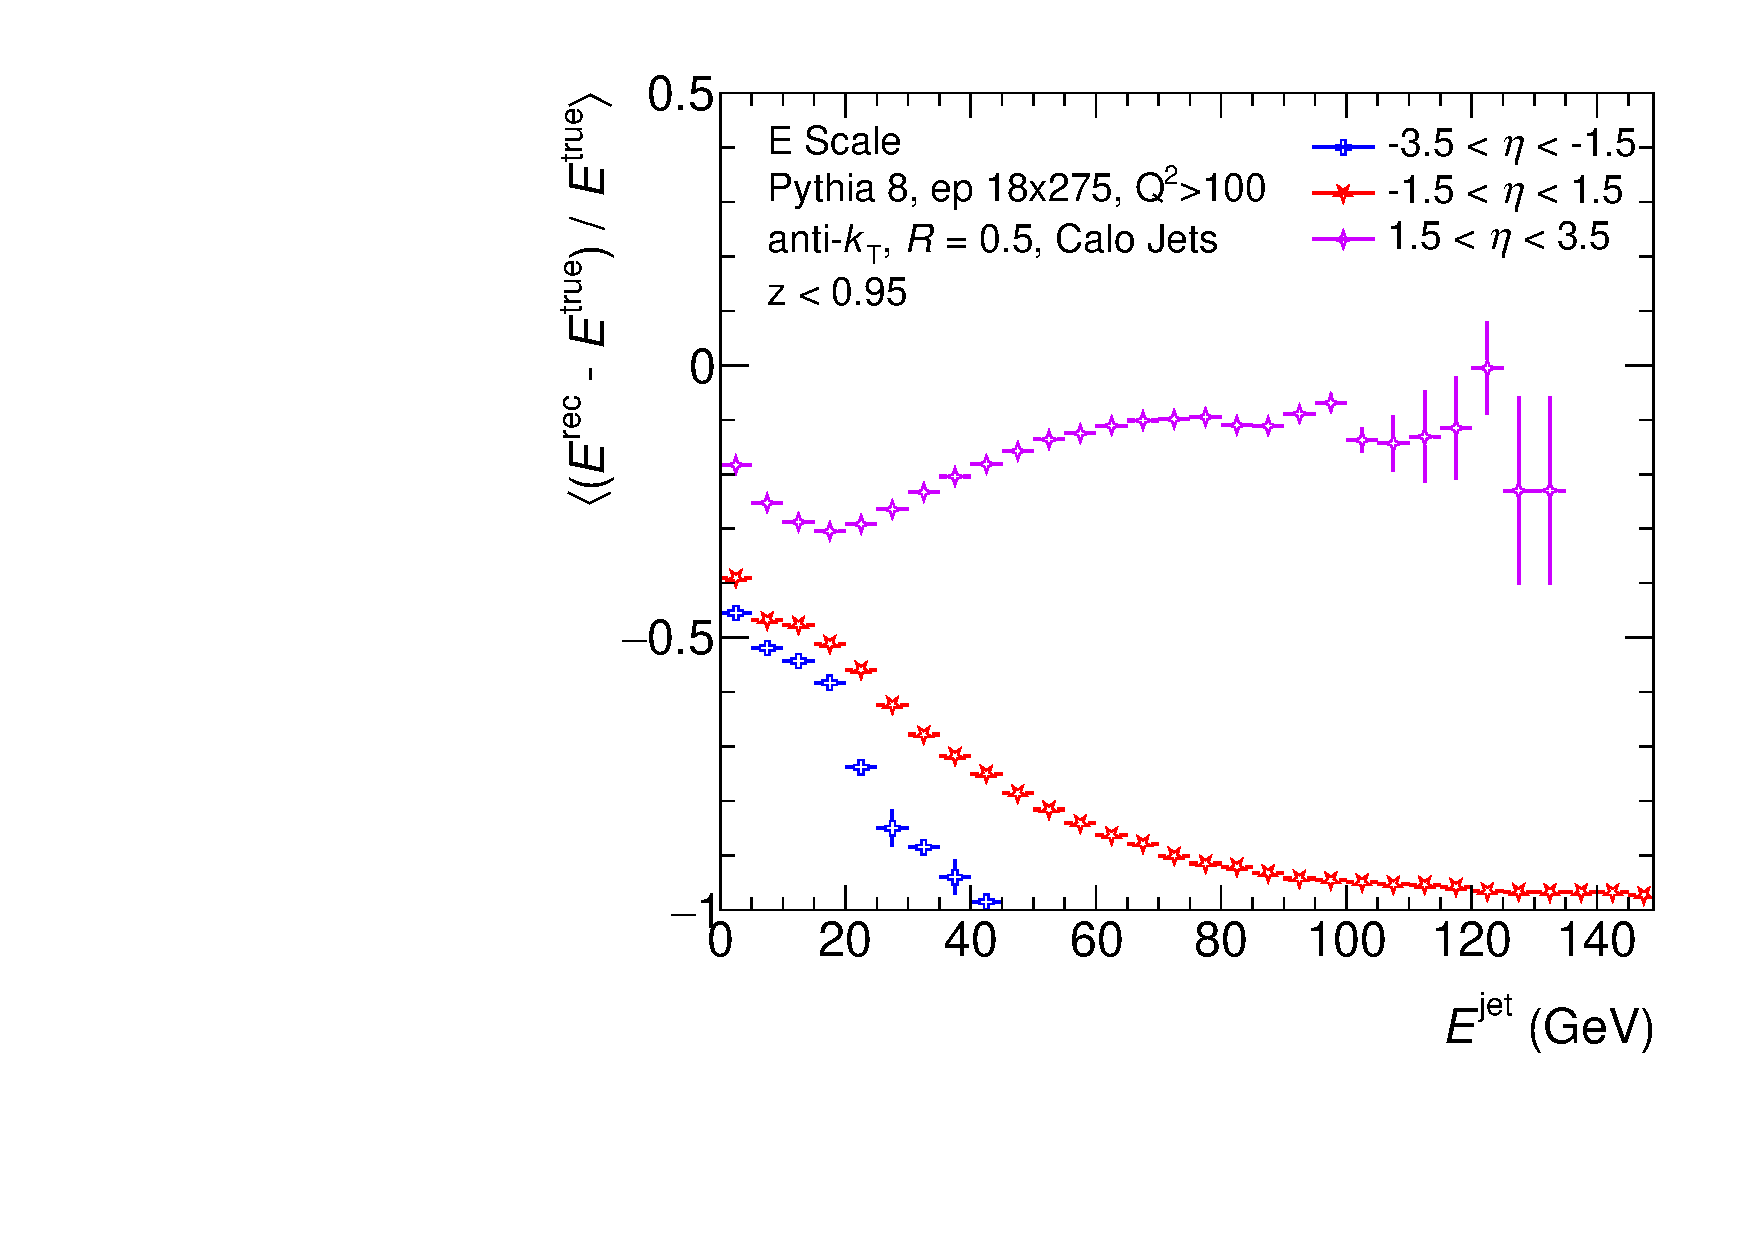
\includegraphics[width=\linewidth]{figs/Final_Plots/JES_calo_grouped.pdf}
        \caption{Calorimetry jets scale, using both hadronic and electromagnetic calorimeters.  The scale for the forward region is good, within 15\% at energies above 50 GeV.  The central and backward regions are areas where the tuning of calorimeter clustering and calibration is still ongoing, thus the poor scale.}
        \label{fig:calo_energy_scale}
    \end{subfigure}
    \hfill
    \begin{subfigure}{0.4\textwidth}
        \centering
        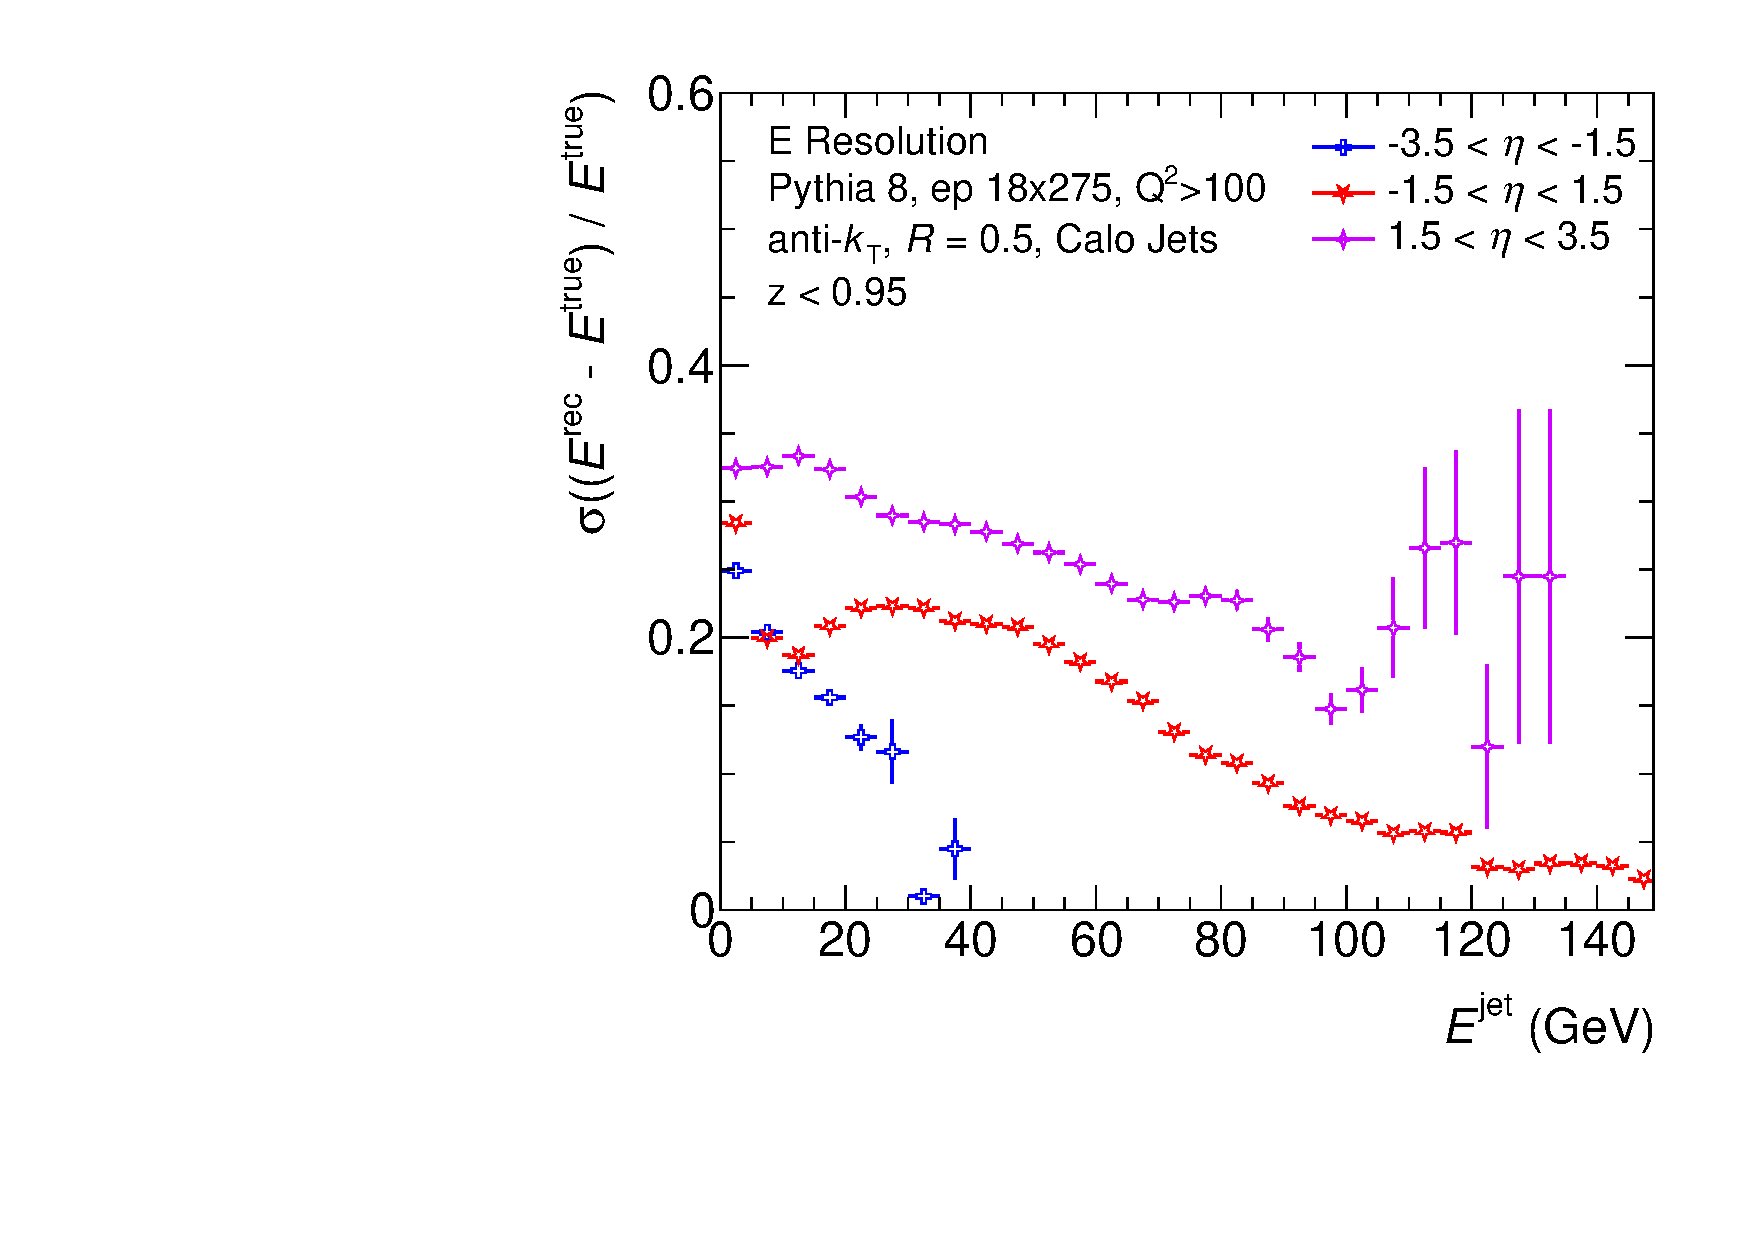
\includegraphics[width=\linewidth]{figs/Final_Plots/JER_E_calo_grouped.pdf}
        \caption{Calorimetry jet resolution.  Despite the poor scale in the central and backward region, the resolution remains good, indicating a small distribution of reconstructed energies for a particular truth energy.}
        \label{fig:calo_energy_resolution}
    \end{subfigure}
    \caption{The scale and resolution of the energy of calorimetry jets.}
    \label{fig:calo_energy_reso_scale}
\end{figure}



\begin{figure}
    \centering
    \begin{subfigure}{0.4\textwidth}
        \centering
        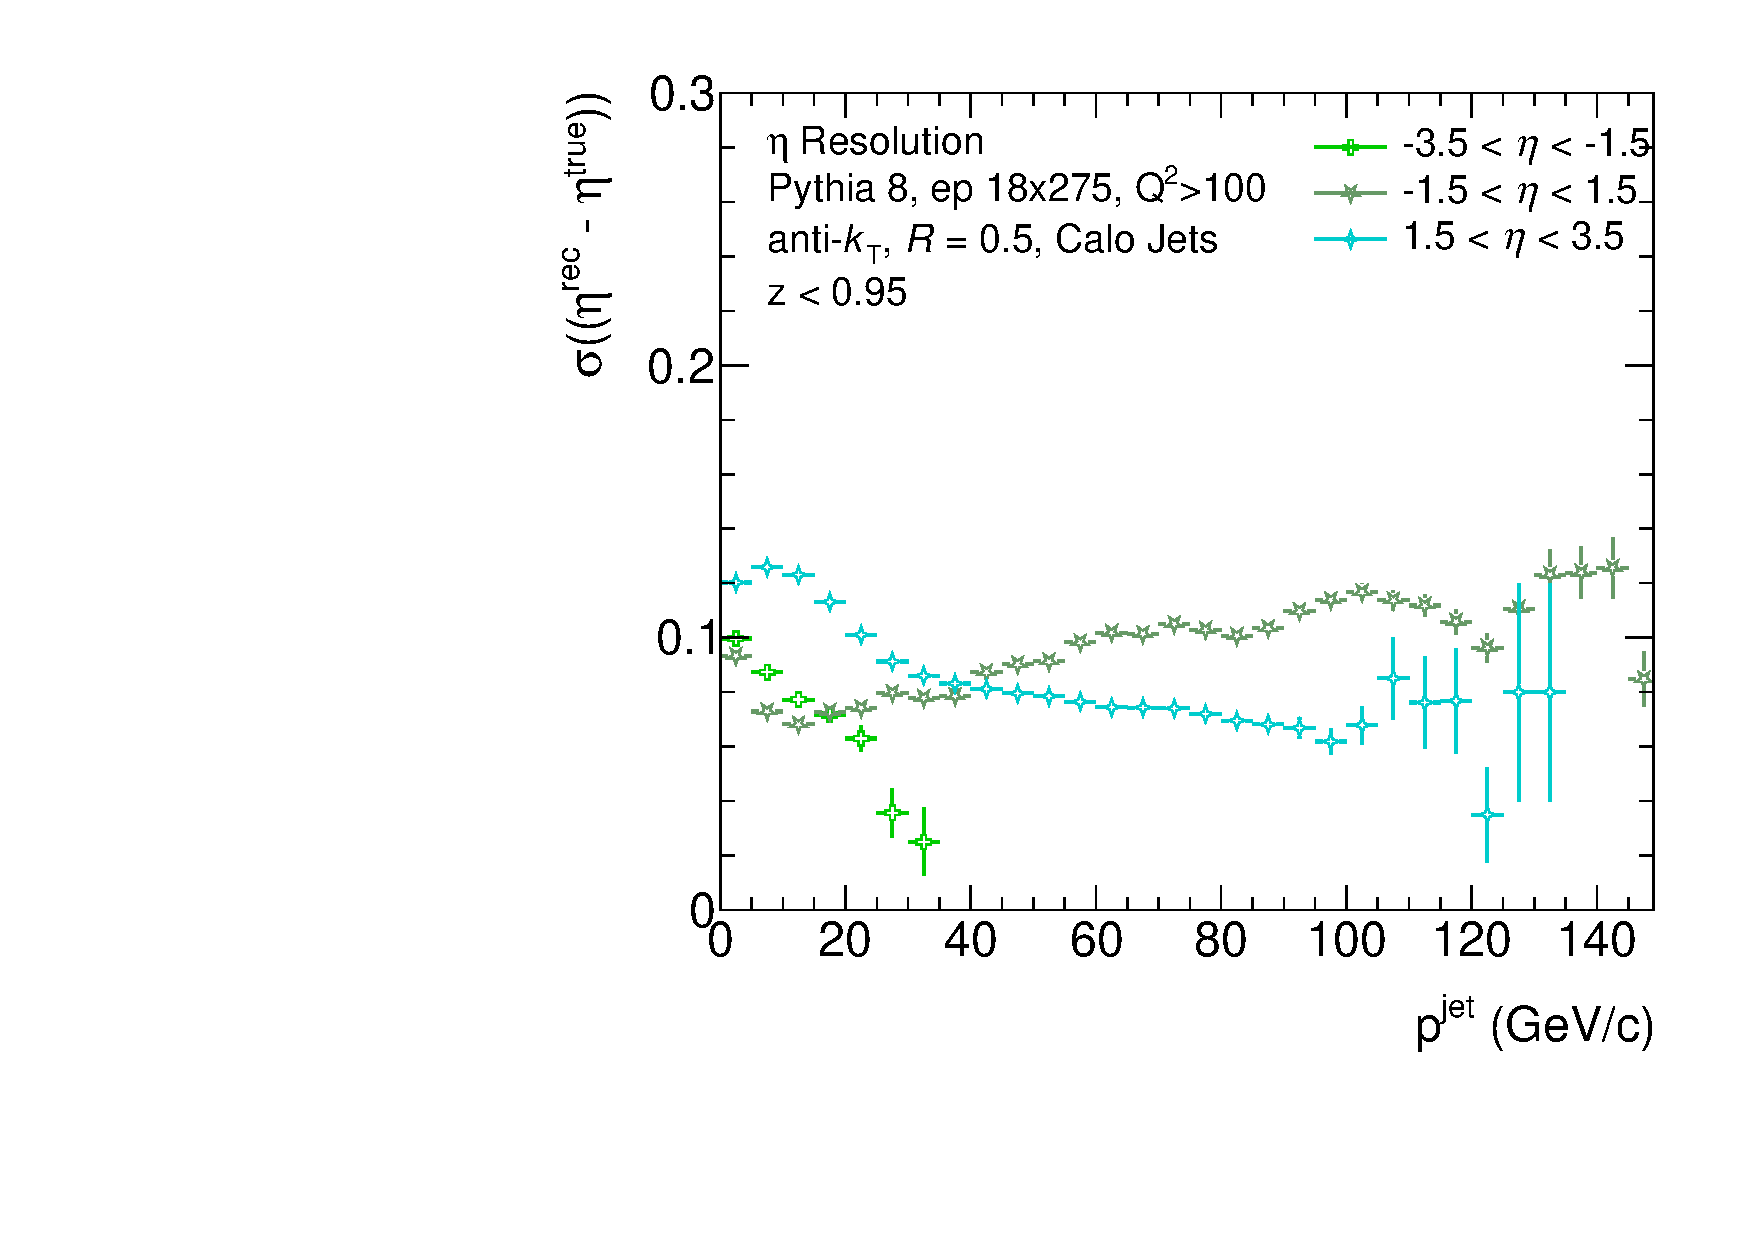
\includegraphics[width=\linewidth]{figs/Final_Plots/EtaReso_calo_grouped.pdf}
        \caption{Calorimetry jet $\eta$ resolution}
        \label{fig:calo_eta_resolution}
    \end{subfigure}
    \hfill
    \begin{subfigure}{0.4\textwidth}
        \centering
        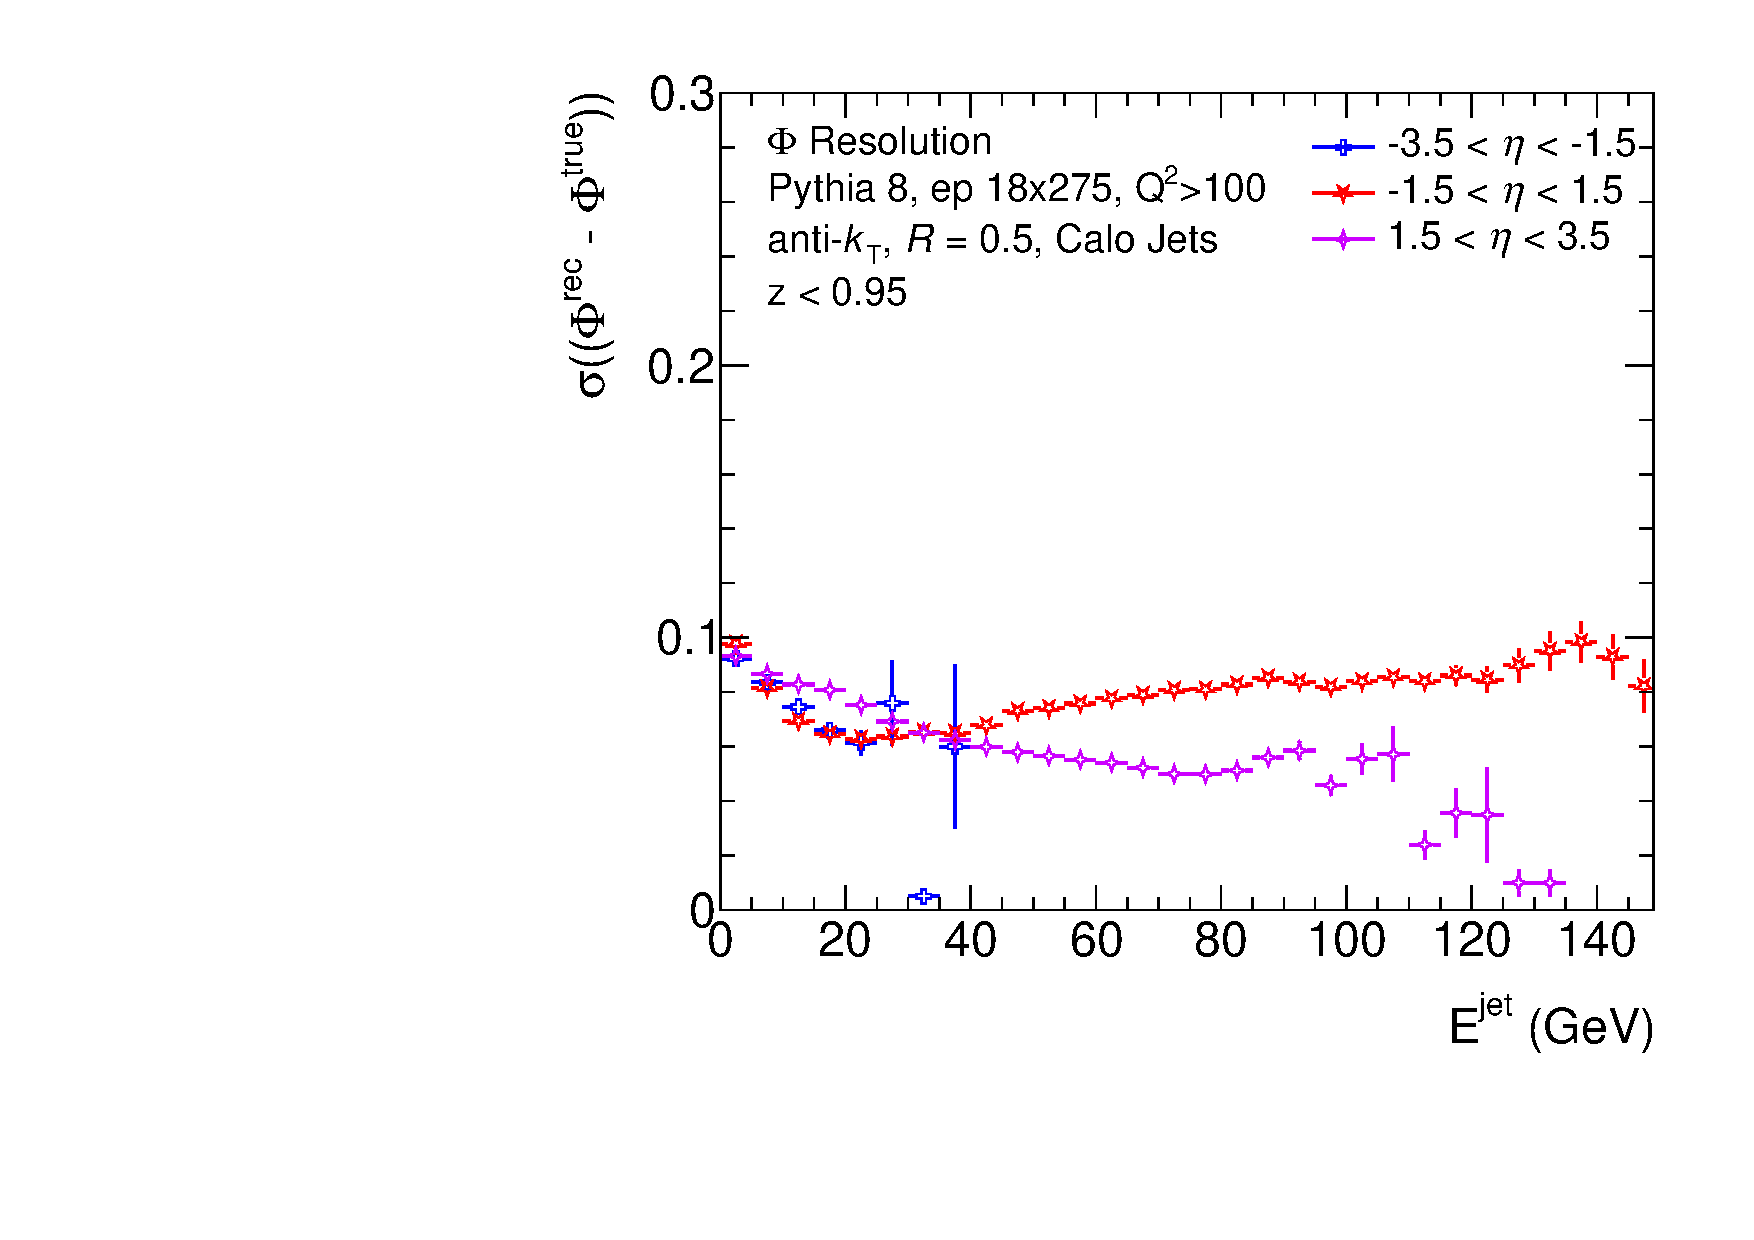
\includegraphics[width=\linewidth]{figs/Final_Plots/PhiReso_calo_grouped.pdf}
        \caption{Calorimetry jet $\phi$ resolution}
        \label{fig:calo_phi_resolution}
    \end{subfigure}
    \caption{The spatial resolution of calorimetry jets.  Since jet matching is done in $\eta-\phi$ space, the poor energy scale for the central and backward regions should have a minimal affect on the spatial resolution.}
    \label{fig:calo_spatial_reso_scale}
\end{figure}
